\documentclass[conference]{IEEEtran}
\usepackage{amsmath,amssymb}
\usepackage{graphicx}
\usepackage{booktabs}
\usepackage{siunitx}
\usepackage{cite}
\usepackage[hidelinks]{hyperref}
\graphicspath{{../results/}}
\sisetup{group-digits=false}
\setlength{\textfloatsep}{8pt plus 2pt minus 2pt}
\setlength{\floatsep}{6pt plus 2pt minus 2pt}
\setlength{\abovedisplayskip}{4pt}\setlength{\belowdisplayskip}{4pt}

\begin{document}
\title{Electromechanical Modes and Fault Response\\of the Kundur Two-Area System}
\author{\IEEEauthorblockN{Haoran Liu}
\IEEEauthorblockA{CloudDRTS preparation, Phase 1}}
\maketitle

\begin{abstract}
The two-area, four-machine benchmark system is modelled with six-state synchronous machines, subjected to a three-phase fault and linearized numerically. The inter-area mode lies at \SI{0.5447}{Hz} with \SI{3.58}{\percent} damping and the two local modes at \SI{1.0806}{Hz} and \SI{1.1113}{Hz}. With the machine model and the saturation treatment of the textbook example, its 22 nonzero eigenvalues are reproduced within \SI{0.012}{s^{-1}}. On the network of Klein, Rogers and Kundur, the computed inter-area frequencies of all four published cases are 3.6--\SI{4.0}{\percent} higher than published and the damping ratios agree within 0.5 percentage points; the mode shape agrees with the published one.
\end{abstract}
\begin{IEEEkeywords}
Inter-area oscillation, modal analysis, small-signal stability, two-area system.
\end{IEEEkeywords}

\section{Introduction}
The two-area system of Kundur~\cite{kundur} is the standard benchmark for inter-area oscillations~\cite{klein} and serves as the reference system for the partitioning studies that follow. This note computes its fault response and electromechanical modes and compares them with~\cite{kundur} and~\cite{klein}.

\section{Model and Method}
\subsection{Network and operating point}
Network, load and machine data are those of~\cite[Example 12.6]{kundur}: 11 buses, four \SI{900}{MVA} units, two \SI{110}{km} tie sections of two circuits each, loads of $967+j100$ and $1767+j100$~MVA at buses 7 and 9, and 200 and \SI{350}{Mvar} of shunt capacitors. Units G2--G4 generate 700, 719 and \SI{700}{MW}, and G1 is the slack unit. The power flow converges to a residual of $2.5\times10^{-12}$~p.u., with \SI{400}{MW} transferred from area~1 to area~2.

\subsection{Machine and load models}
Each unit is a round-rotor model with the six states $\delta$, $\Delta\omega$, $e'_q$, $e'_d$, $\psi_{1d}$ and $\psi_{2q}$, the swing equations $\dot\delta=\omega_0\Delta\omega$, $2H\Delta\dot\omega=T_m-T_e$ and the flux equations of~\cite{kundur}. Field voltage and mechanical torque are constant, and saturation is neglected unless stated otherwise. Active load is modelled as constant current and reactive load as constant impedance; the network equations with these loads are solved by Newton's method at every evaluation of the state derivatives $\dot x=f(x)$.

\subsection{Linearization and mode identification}
The state matrix is formed by central differences at the equilibrium $x_0$,
\begin{equation}
A_{:,j}=\frac{f(x_0+h\,e_j)-f(x_0-h\,e_j)}{2h},\qquad h=10^{-5},
\end{equation}
where $\lVert f(x_0)\rVert_\infty=1.7\times10^{-12}$; halving $h$ changes no eigenvalue by more than \SI{e-9}{s^{-1}}. For an eigenvalue $\lambda=\sigma\pm j\omega$ the frequency is $\omega/2\pi$ and the damping ratio $\zeta=-\sigma/|\lambda|$. The rotor modes are those with $1<\omega<\SI{12}{rad/s}$. With $\hat v$ the speed mode shape of G1--G4 normalized to its largest entry, a mode is labelled inter-area if
\begin{equation}
\Bigl|\tfrac{\hat v_1+\hat v_2}{2}-\tfrac{\hat v_3+\hat v_4}{2}\Bigr|>\max\bigl(|\hat v_1-\hat v_2|,\,|\hat v_3-\hat v_4|\bigr),
\end{equation}
and local to the area with the larger internal difference otherwise.

\section{Results}
\subsection{Electromechanical modes}
\begin{table}[!t]
\caption{Rotor Modes, Given as $f$ (Hz) / $\zeta$ (\%)}
\label{tab:modes}
\centering\footnotesize\setlength{\tabcolsep}{3pt}
\begin{tabular}{@{}lccc@{}}
\toprule
Mode & No saturation & Method of~\cite{kundur} & \cite{kundur}, Table E12.3\\
\midrule
Inter-area & 0.5447 / 3.58 & 0.5454 / 3.23 & 0.545 / 3.2\\
Local, area 1 & 1.0806 / 8.52 & 1.0873 / 7.18 & 1.087 / 7.2\\
Local, area 2 & 1.1113 / 8.41 & 1.1175 / 7.19 & 1.117 / 7.2\\
\bottomrule
\end{tabular}
\end{table}
\begin{figure}[!t]
\centering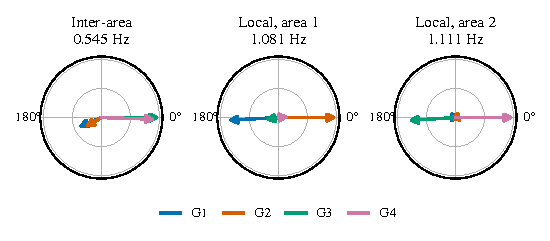
\includegraphics[width=\columnwidth]{phase1_mode_shapes.pdf}
\caption{Speed mode shapes of the rotor modes, normalized to the largest entry.}
\label{fig:modes}
\end{figure}
Table~\ref{tab:modes} and Fig.~\ref{fig:modes} give the three rotor modes. In the inter-area mode G1 and G2 swing against G3 and G4; in each local mode the two units of one area swing against each other, as in~\cite{kundur}.

The frequencies agree with~\cite{kundur} within \SI{0.6}{\percent}, while the local modes are about 1.3 percentage points better damped. The difference is due to saturation. Example 12.6 includes saturation ($A_\mathrm{sat}=0.015$, $B_\mathrm{sat}=9.6$, $\psi_{T1}=0.9$), and its small-signal analysis uses an equivalent-circuit machine model in which saturation is linearized with the incremental factor $1/(1+B_\mathrm{sat}\psi_I)$ on both axes. Without saturation this model has the same eigenvalues as the six-state model (within \SI{3e-4}{s^{-1}}). With the saturation treatment of~\cite{kundur} (third column of Table~\ref{tab:modes}), the 22 nonzero eigenvalues of Table E12.3 are reproduced within \SI{0.012}{s^{-1}}. With the thyristor exciter of Table E12.4 ($K_A=200$, $T_R=\SI{0.01}{s}$) the inter-area mode becomes unstable, $+0.030\pm j3.84$ against $+0.031\pm j3.84$ in~\cite{kundur}, and the case with transient gain reduction agrees within \SI{0.005}{s^{-1}}. With the power system stabilizer, differences of up to \SI{0.10}{s^{-1}} remain unexplained.

Without saturation the model also has a slow real eigenvalue at $+\SI{0.0049}{s^{-1}}$ (time constant about \SI{200}{s}); with the saturation treatment of~\cite{kundur} all eigenvalues except the pair at the origin are stable. Started on the real part of each mode shape (amplitude $10^{-4}$), the nonlinear model follows $\mathrm{Re}(v\,e^{\lambda t})$ over \SI{5}{s} within \SI{0.5}{\percent} of the initial displacement, which confirms the linearization.

\subsection{Fault response}
\begin{figure}[!t]
\centering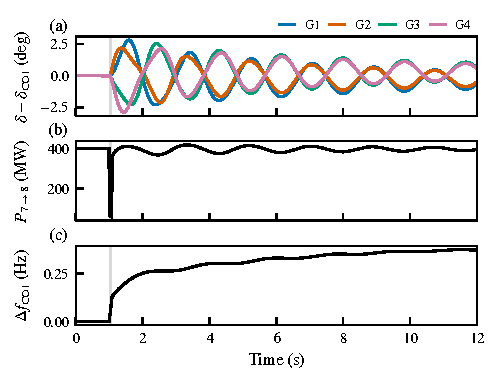
\includegraphics[width=\columnwidth]{phase1_fault.pdf}
\caption{Three-phase fault at bus 8, \SIrange{1.00}{1.08}{s} (shaded): (a) rotor angles relative to the centre of inertia (COI), (b) power from bus 7 to bus 8, (c) COI frequency deviation.}
\label{fig:fault}
\end{figure}
A three-phase fault ($R_f=10^{-4}$~p.u.) is applied at bus~8, in the middle of the tie, from 1.00 to \SI{1.08}{s}. The equations are integrated with DOP853 (relative tolerance $10^{-8}$), restarted at both switching instants. The largest pre-fault speed deviation, \SI{3e-13}{Hz}, confirms a consistent initial state. During the fault the bus-8 voltage falls to 0.0016~p.u. and the tie power from 400 to about \SI{65}{MW} (Fig.~\ref{fig:fault}). After clearing, the response is dominated by the slowly decaying \SI{0.54}{Hz} inter-area swing, with the local modes visible during the first two seconds. Without governors the energy imbalance during the fault is not corrected, and the COI frequency ends \SI{0.37}{Hz} above nominal, so the rotor angles are shown relative to the COI.

\section{Comparison With Klein, Rogers, and Kundur}
\begin{table}[!t]
\caption{Inter-Area Mode of the Symmetric Zero-Transfer Cases of~\cite{klein}, Given as $f$ (Hz) / $\zeta$ (\%)}
\label{tab:klein}
\centering\footnotesize\setlength{\tabcolsep}{4pt}
\begin{tabular}{@{}lccc@{}}
\toprule
Excitation, ties & \cite{klein} & This model & $\Delta f$\\
\midrule
Manual, 1 & 0.481 / 2.3 & 0.499 / 1.9 & $+\SI{3.6}{\percent}$\\
Static, 1 & 0.513 / 0.2 & 0.534 / 0.7 & $+\SI{4.0}{\percent}$\\
Static, 2 & 0.661 / 1.1 & 0.687 / 1.6 & $+\SI{3.9}{\percent}$\\
Static, 3 & 0.748 / 1.8 & 0.776 / 2.2 & $+\SI{3.7}{\percent}$\\
\bottomrule
\end{tabular}
\end{table}
Reference~\cite{klein} reports only the inter-area mode. Its Table 2 gives \SI{0.481}{Hz} and $\zeta=0.023$ for the symmetric system (\SI{1400}{MW} of generation and \SI{1367}{MW} of constant-impedance load per area, no transfer) with manual excitation and one tie circuit; its Table 1 gives the same mode with fast static exciters ($K_A=200$, $T_R=\SI{0.01}{s}$) for three, two and one tie circuits. That Table 1 uses exciters without transient gain reduction follows from its one-circuit value, which equals the corresponding entry of Table 2. The network of~\cite[Fig.~1]{klein} has the line data of the textbook network but no step-up transformers; the units are connected directly to their buses, all units have $H=\SI{6.5}{s}$, and shunt capacitors are only said to have been added as necessary. These four cases are computed for this network with \SI{200}{Mvar} per area.

Table~\ref{tab:klein} shows that all four frequencies are 3.6--\SI{4.0}{\percent} higher than published, and that the damping ratios agree within 0.5 percentage points. The nearly constant ratio, independent of the number of tie circuits and of the exciter type, points to a factor common to all cases rather than to the tie. Data not given in~\cite{klein} were varied to check this: shunt compensation of 100 or \SI{300}{Mvar} per area, or neglecting line charging, changes the frequencies by at most \SI{1.1}{\percent}, and neglecting line resistance by at most \SI{2.6}{\percent}. None of these variations removes the offset in all four cases; the remaining offsets range from 0.9 to \SI{5.2}{\percent}. The mode shape agrees with~\cite[Fig.~2]{klein}: the units of one area swing in exact anti-phase with those of the other, and the outer units G1 and G3 oscillate with a larger amplitude than the inner units (ratio 0.91). For reference, the textbook network with its 0.15~p.u. step-up transformers gives frequencies \SIrange{4.9}{11.5}{\percent} below~\cite{klein}.

\section{Conclusion}
The model reproduces the textbook modes with the saturation treatment of~\cite{kundur}. On the network of~\cite{klein}, damping ratios and mode shape agree, while the inter-area frequency is systematically about \SI{4}{\percent} higher; the cause has not been identified from the published data. The textbook network, whose data are complete, is proposed as the reference for the partitioned studies.

\begin{thebibliography}{1}
\bibitem{kundur} P.~Kundur, \emph{Power System Stability and Control}. New York: McGraw-Hill, 1994.
\bibitem{klein} M.~Klein, G.~J. Rogers, and P.~Kundur, ``A fundamental study of inter-area oscillations in power systems,'' \emph{IEEE Trans. Power Syst.}, vol.~6, no.~3, pp.~914--921, Aug. 1991.
\end{thebibliography}
\end{document}
